\chapter{Incorporating Spatial Effects}
\label{chap4}

\hspace{\parindent} After analysing the model, it was then compared to real-life applause.
The applause duration of varying audience sizes was recorded and graphed. 
Selection criteria for the data included a definite applause time that was fully-recorded and uncut, and a known population. 
Because of this, most of the videos are live concerts and musical performances.
The data points were plotted in different ways in order to find an appropriate linear trend in figure \ref{fig:realclap}.

Figure \ref{fig:realclap} (d) makes the most sense; the applause duration of the audience is dependent on the size of the audience.
The question now is whether or not the compartmental model can recreate \ref{fig:realclap} (d).
Sadly, the current model is scale-free; changing the population does not affect the applause duration for a given set of parameters.
This is because of the assumption that the network is fully connected, meaning that an audience member in front is influenced the exact same way by the whole audience as an audience member at the back.
As this does not seem to be the case in real-life applause, spatial effects must be incorporated by modifying the feedback function $f'(\alpha)$.


\begin{figure}[h]
  \centering
  \begin{subfigure}[b]{0.4\linewidth}
    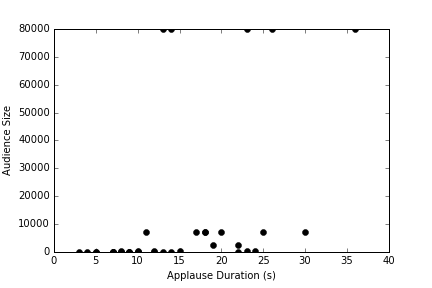
\includegraphics[width=\linewidth]{images/chapter4/1.png}
    \caption{Graphing size versus applause duration.}
  \end{subfigure}
  \begin{subfigure}[b]{0.4\linewidth}
    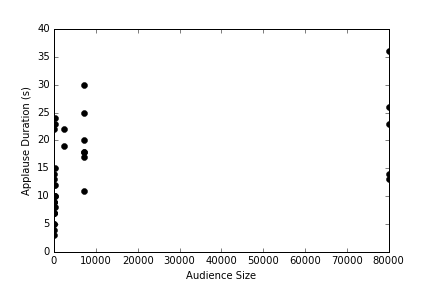
\includegraphics[width=\linewidth]{images/chapter4/2.png}
    \caption{Graphing applause duration versus size.}
  \end{subfigure}
    \begin{subfigure}[b]{0.4\linewidth}
    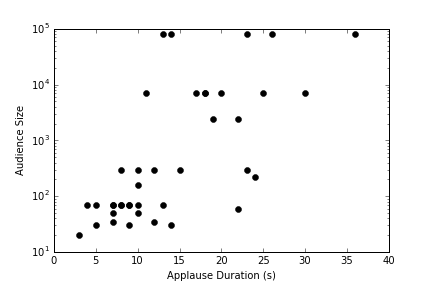
\includegraphics[width=\linewidth]{images/chapter4/3.png}
    %\label{fig:nonTrivSim}
    \caption{Graphing size (in the logarithmic scale) versus applause duration}
  \end{subfigure}
    \begin{subfigure}[b]{0.4\linewidth}
    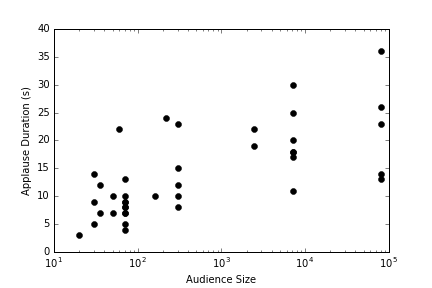
\includegraphics[width=\linewidth]{images/chapter4/4.png}
    %\label{fig:nonTrivSim}
    \caption{Graphing applause duration versus size (in the logarithmic scale).}
  \end{subfigure}
  \caption{Different graphs of the data points of real-life applause.}
  \label{fig:realclap}
\end{figure}


\section{Different configurations for field of vision}

\hspace{\parindent}The field of view configurations represent the audience members that may influence the reference agent.
In real-life, the  reference agent is only influenced by the audience members it can see.
The network is no longer fully-connected, observing a modified, extended Moore neighborhood.
It is extended since it considers all agents till the front row of the system, and not just those $1$ unit away.
Is is modified since it does not consider all directions; the directions considered are affected by the configuration.
'0 degrees' represents all audience members only directly in front of the reference agent until the very front. 
'180 degrees' represents all rows ahead of the reference agent. 
'90 degrees' represents a spatial configuration somewhere in between '0 degrees' and '180 degrees'; considering all agents from the north-east direction to the north-west. The configurations are shown in figure \ref{fig:spaceconfig}.

\begin{figure}[h]
  \centering
  \begin{subfigure}[b]{0.3\linewidth}
    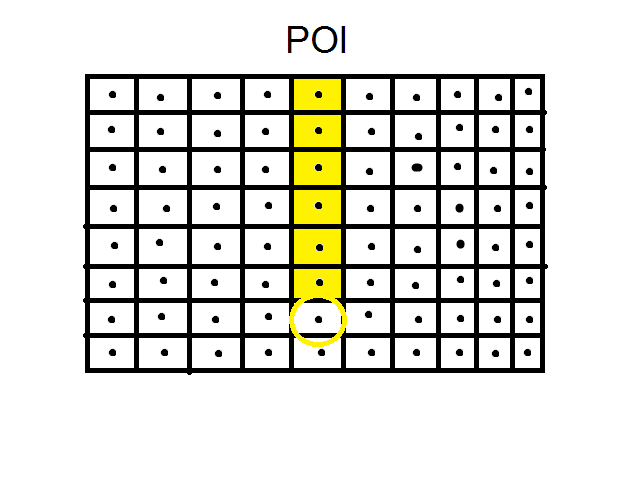
\includegraphics[width=\linewidth]{images/chapter4/0deg.png}
    \caption{'0 degrees'}
  \end{subfigure}
  \begin{subfigure}[b]{0.3\linewidth}
    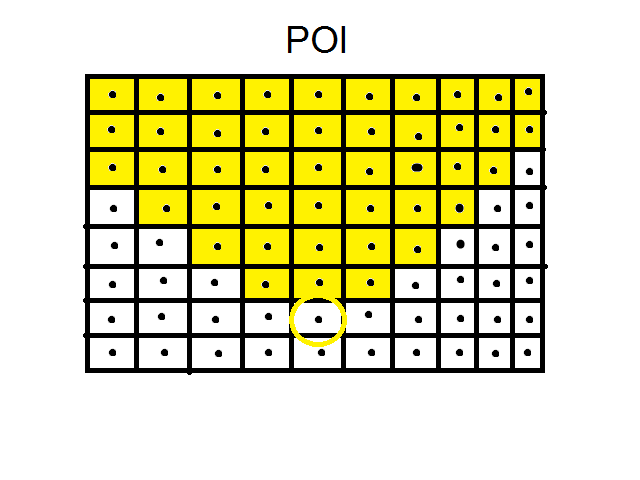
\includegraphics[width=\linewidth]{images/chapter4/90deg.png}
    \caption{'90 degrees'}
  \end{subfigure}
    \begin{subfigure}[b]{0.3\linewidth}
    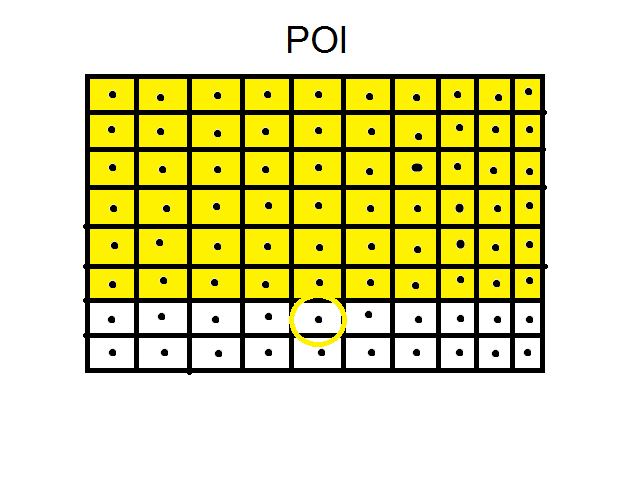
\includegraphics[width=\linewidth]{images/chapter4/180deg.png}
    %\label{fig:nonTrivSim}
    \caption{'180 degrees'}
  \end{subfigure}
  \caption{Different field-of-view configurations. The areas highlighted in yellow are what can influence the  encircled reference agent.}
  \label{fig:spaceconfig}
\end{figure}

\section{Simulating the different spatial configurations}

\hspace{\parindent} Initially, $f'(\alpha)$ bases the fraction of $n_{c}$ throughout the whole population. After incorporating spatial effects, that fraction is only within the field-of-view of the reference agent.
Even after spatial effects, the feedback function is still parametrized by $\alpha$.
The code developed is provided in the appendix (\ref{apndx:spacesim}).

\begin{figure}[h]
  \centering
  \begin{subfigure}[b]{0.3\linewidth}
    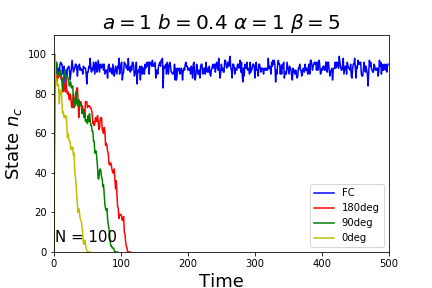
\includegraphics[width=\linewidth]{images/chapter4/feedback_sim4.png}
    \caption{A sample case.}
  \end{subfigure}
  \begin{subfigure}[b]{0.3\linewidth}
    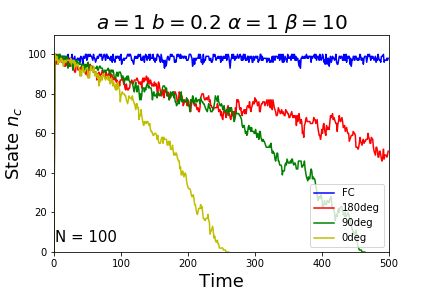
\includegraphics[width=\linewidth]{images/chapter4/feedback_sim5.png}
    \caption{A sample case.}
  \end{subfigure}
    \begin{subfigure}[b]{0.3\linewidth}
    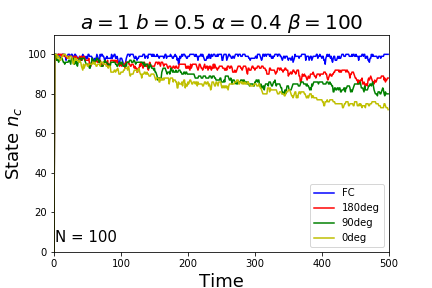
\includegraphics[width=\linewidth]{images/chapter4/feedback_sim6.png}
    %\label{fig:nonTrivSim}
    \caption{A sample case.}
  \end{subfigure}
    \begin{subfigure}[b]{0.3\linewidth}
    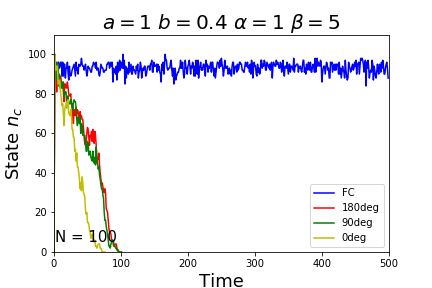
\includegraphics[width=\linewidth]{images/chapter4/feedback_sim3.png}
    %\label{fig:nonTrivSim}
    \caption{A case where '90 degrees' is similar to '0 degrees'.}
  \end{subfigure}
    \begin{subfigure}[b]{0.3\linewidth}
    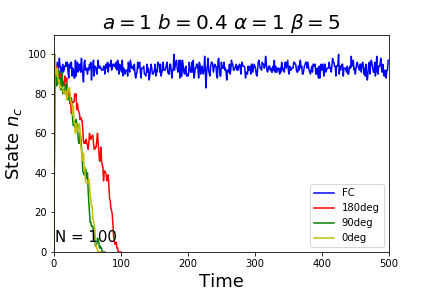
\includegraphics[width=\linewidth]{images/chapter4/feedback_sim2.png}
    %\label{fig:nonTrivSim}
    \caption{A case where '90 degrees' is similar to '180 degrees'.}
  \end{subfigure}
  \begin{subfigure}[b]{0.3\linewidth}
    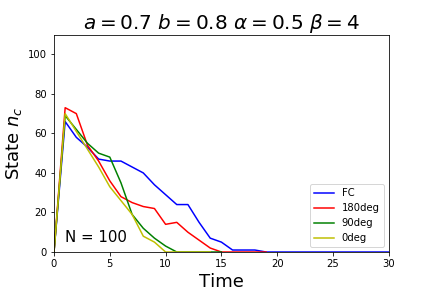
\includegraphics[width=\linewidth]{images/chapter4/feedback_sim7.png}
    %\label{fig:nonTrivSim}
    \caption{A case where all configurations have a trivial steady-state $0$.}
  \end{subfigure}
  \caption{Different graphs comparing effect of different feedback functions under different parameters.}
  \label{fig:spacesim}
\end{figure}

Shown in figure \ref{fig:spacesim} are simulations with different parameters ($a,b,\alpha,\beta$) comparing the different feedback functions, the original fully-connected network, '180 degrees', '90 degrees', and '0 degrees'.
Graphs (a), (b), and (c) show that in our system feedback functions are less effective in less connected networks. 
There is clearly a downward trend (starting from FC, '180', '90', then '0') when it comes to applause duration.
Graphs (d) and (e) show that '90 degrees' can be similar to either remaining configurations, as well as be somewhere in between.
Generally, simulations incorporating any form of field-of-view feedback do not have a non-trivial steady-state.
Graphs (b) and (c) show cases where the simulations have not ended, but exhibit an obvious downward trend.
Given more iterations, the simulations would end, unlike the fully-connected ones.
Graph (g) shows a special case where all simulations have a trivial steady-state of zero.
One thing to note is that the analysis done for the fully-connected system (phase space graphs, critical and unstable points) cannot be applied to the systems with spatial effects.
A different steady-state equation must be setup to reflect how each agent is influenced differently.
Such analysis will no longer be pursued as it is outside the skill set of the researcher.

\section{Finding the parameters $(a,b,\alpha,\beta)$ for real-life applause}

\hspace{\parindent}Recalling, incorporating spatial effects to the feedback function effectively reduces the number of agents influencing a reference agent. Increasing the population size should increase the feedback since the agents in the back row of a 100x100 grid should 'see' more people than those in the back row of a 10x10 grid. 
This effectively eliminates the original problem of the fully-connected network being scale free.
It is now possible for the applause duration to be dependent on the population.
This phenomena is investigated by simulating a set of parameters $(a,b,\alpha,\beta)$ with varying populations.
For simplicity, the system grid will always be a 2-dimensional lattice of equal lengths.
Also, the spatial configuration used will be '180 degrees'.
The total population sample will be perfect squares ranging from $10^1$ to $10^4$.
The code developed is provided in the appendix (\ref{apndx:popdep}).